\documentclass[12pt,a4paper,oneside]{article}
\title{Využití šifer v informační komunikační technologii}
\author{Cyril Steger}
\date{12.2.2024}
% Polyglossia 
\usepackage{polyglossia}
\setdefaultlanguage{czech}
\usepackage{fontspec}
\setmainfont{Times New Roman} % nebo jiný font

% Matematické znaky
\usepackage{amsmath}        
\usepackage{amsfonts}       

% Obrazky
\usepackage{graphicx}
\newcommand{\FIGURES}{./img} %cesta k adresáři s obrázky
\newcommand{\CHAPTERS}{./src} %cesta k adresáři s kapitolami

% Bibtex 
\usepackage[backend=biber,style=iso-authoryear, autolang=other, maxnames=2, minnames=1]{biblatex}
\addbibresource{references.bib}

% Typograficke minimum
\usepackage{csquotes} % doporučuje se pro biblatex
\usepackage{microtype}
\usepackage{parskip} % odstavce bez odsazení, ale s odstupem
\setlength{\parindent}{0pt}    % Žádné odsazení
\setlength{\parskip}{1em}      % Svislá mezera mezi odstavci
\hyphenpenalty=1000  % Mírná penalizace za dělení slov
\widowpenalty=10000   % Zákaz vdov a sirotků
\emergencystretch=1.5em % Mírně tolerantnější mezery

% Nastaveni odkazu
\usepackage[unicode]{hyperref} % generovani odkazu v PDF
\hypersetup{pdftitle=Využití šifer v informační komunikační technologii, 
            pdfauthor=Cyril Steger,
            colorlinks=false,
            urlcolor=blue,
            pdfstartview=FitH,
            pdfpagemode=UseOutlines,
            pdfnewwindow,
            breaklinks  %% zajistí, aby se dlouhé hyperodkazy mohly lámat přes více řádků
}
\usepackage[nottoc]{tocbibind} % Automatické přidaní seznamu literatury do /printbibliography

\begin{document}

%Titulní strana
\pagestyle{empty}
\begin{center}
    
    {\large Technická univerzita v Liberci}

    \medskip
    {\large Ekonomická fakulta}
    %logo
    \vfill
    \centerline{\mbox{
\includegraphics[width=55mm]{\FIGURES/tul-ef_symbol_colour_RGB.png}}} %logo
    \vfill
    \vspace{5mm}
    %title cz
    {\LARGE\bfseries Využití šifer v informační komunikační technologii}
    %title en
    \vspace{5mm}
    {\large Usage of Cryptography in information communication technology}

    \vfill
    \vspace{5mm}
    {\large Cyril Steger}
    
    \vfill
    \begin{tabular}{rl}
        Vedoucí seminární práce: &  Ing. David Kubát, Ph.D.\\   %% Jméno a příjmení s~tituly 
        \noalign{\vspace{2mm}}
        Studijní program: & Systémové inženýrství a informatika\\
        \noalign{\vspace{2mm}}
        Studijní obor: & Navazující studium prezenční\\
        \noalign{\vspace{2mm}}
    \end{tabular}
    \medskip

    \vfill
    {\large Liberec 2024}
    
\end{center}
%Obsah
\newpage
\pagestyle{plain}
\setcounter{page}{1} %Nastavení číslování stránek

\tableofcontents

%Kapitoly
%Uvod
\hyphenation{ko-mu-ni-kač-ních}
\section {Úvod}
Tématem této seminární práce je použití šifer v oblasti informačních a komunikačních technologií (dále jen ICT). Kryptografie, jako vědní disciplína, hraje klíčovou roli při zajišťování bezpečnosti a ochrany dat nejen v digitálním světě, kde je bezpečný přenos informací nezbytný pro každodenní komunikaci a sdílení informací. Cílem této práci je seznámit čtenáře se základními pojmy používané v dnešní kryptografii a zvýšit tak povědomí o tom kde a jak je v dnešní oblasti ICT využívána.

V první části nás práce stručně seznámí s historií a základními pojmy používanými v oblasti kryptografie, které jsou důležité k pochopení pro následující kapitoly. Nejprve bude představena Shannonova teorie informace, která tvoří teoretický základ moderní kryptografie a komunikačních systémů. Tato teorie je zásadní pro pochopení principů šifrování a bezpečné výměny dat.

Další část práce je rozdělena do tří hlavních kapitol, z nichž každá se zaměřuje na jednu z kategorií šifer používaných v současné kryptografii. První kategorie jsou symetrické šifry, též známé jako šifry s tajným klíčem. Následující kapitola se věnuje asymetrickým šifrám, kde bude podrobně vysvětlena šifra RSA, která je jedním z nejpoužívanějších šifer s veřejným klíčem \parencite{drake2024}. Poslední kategorií jsou hybridní šifry, které kombinují výhody symetrických a asymetrických šifer a jsou využívány v mnoha moderních komunikačních protokolech.

Závěrem se práce bude věnovat oblasti postkvantové kryptografie, která se zabývá vývojem šifrovacích algoritmů odolných vůči kvantovým počítačům. V této části se seznámíme s aktuálními výzvami a vývojem v oblasti kryptografie, včetně Shorova algoritmu, který představuje hrozbu pro současné asymetrické šifry, zejména RSA.
\newpage
%Kryptografie
\section{Kryptografie}
Kryptografie je vědní disciplína zaměřená na ochranu informací. Cílem kryptografie je zajistit, aby určité informace zůstaly skryté před neoprávněnými osobami. K tomu využívá různé metody a techniky, které zajišťují nejen důvěrnost dat, ale také jejich autentičnost. Kryptografie se dále zaměřuje na prevenci neautorizovaných změn v datech, zajišťuje, že odesílatel nemůže popřít svůj podpis nebo provedení akce, a chrání informace před jejich zneužitím. Využívá se tedy pro zajištění bezpečnosti a integrity informací nejen v digitálním světě \parencite{tesar2021}.

Kryptografie primárně vznikla k ochraně zpráv během jejich přenosu a tak až donedávna byly její doménou přenosové systémy. Později se ukázalo, že matematické metody lze použít nejen k utajování obsahu zpráv, ale rovněž k zajištění bezpečnosti mnoha dalších systémů. Mezi ně patří například systém řízení přístupu, elektronických plateb, síťových protokolů apod. S aplikacemi kryptografie proto přicházíme do styku každý den, avšak všeobecné povědomí o tom, jak fungují a na čem jsou založené, je nízké \parencite{burda2019}.

Jak již bylo uvedeno, v dnešním světě se kryptografie nejvíce soustředí na komunikaci mezi přenosovými kanály, ke kterému mají kromě autora zprávy a adresáta přístup i jiné (neoprávněné) osoby. Některé z těchto osob totiž usilují o čtení, resp. pozměňování přenášených zpráv a získat tak co nejvíce (citlivých) informací. Kryptografické techniky, které budou více rozebrány v této práci, umožňují autorovi a adresátovi zajistit ochranu přenášených zpráv před těmito hrozbami \parencite{sedlak2021}.

\subsection{Historie}

V počátcích internetu se šifrování prakticky nevyužívalo, protože větší důraz byl kladen na ochranu citlivých informací tajných orgánů států. Síť tehdy používala otevřené pakety, které byly přenášeny pomocí protokolů, jež, i když byly postupně upravovány, jsou používány stále v současnosti. To znamenalo, že veškerá komunikace probíhala v otevřeném textu, což umožňovalo snadné odposlechy a manipulaci s daty \parencite{erben2014}.

Například protokol FTP (File Transfer Protocol), který byl navržen v roce 1985 v dokumentu RFC 959, neobsahoval žádnou podporu pro šifrování. Obsah zpráv, stejně jako řídicí informace - například uživatelské jméno a heslo sloužící k připojení - byly snadno dostupné pro třetí stranu. S postupným rozvojem internetu a dostupností široké veřejnosti se začaly objevovat i první vážné problémy s jeho bezpečností \parencite{cerna2012}.

První vážné problémy s bezpečností v síti se objevily v roce 1989, kdy počítačový červ WANK (Worms Against Nuclear Killers) napadl systémy NASA. Po infikování systému zobrazoval při přihlášení politicky motivovanou zprávu, která kritizovala jaderný program a plánovaný start sondy Galileo. I když červ data nepoškozoval, jeho hlavním cílem bylo šíření anti-jaderného poselství a byl jedním z prvních virusů s tímto motivem vydírání \parencite{erben2014}.

Dalším případem je útok na americkou banku Citibank, na kterou se zaměřil ruský hacker Vladimir Levin. Celkem jednoduše získal přístup k účtům významných korporátních klientů a pokusil se převést přibližně 10,7 milionu dolarů na účty svých kompliců. Tento incident vyvolal mezinárodní pozornost, upozornil na zranitelnosti elektronického bankovnictví a vedl k posílení bezpečnostních opatření v bankovním sektoru \parencite{erben2014}.

Bylo jasné, že pokud má internet stát běžně používanou komunikační platformou, je nezbytné zaměřit se na zabezpečení přenosu informací, tedy na šifrování. Šifrování internetového provozu se dnes stalo standardem a jeho implementace se nejčastěji provádí prostřednictvím protokolu SSL/TLS nebo S/MIME pro bezpečnou elektronickou poštu \parencite{pavlicek2012}. Tyto síťové protokoly využívají asymetrickou kryptografii, což je podrobněji vysvětleno v kapitole \hyperref[sec:asymetricka-kryptografie]{Využití Asymetrických šifer}.

I když jsou z matematického hlediska šifry prakticky neprolomitelné, největším současným problémem zůstává sociální (mezilidský) aspekt - otázka důvěry. V praxi to znamená, že si každá ze stran komunikace musí klást otázku: „Je protistrana opravdu tím, za koho se vydává?“ Ve fyzickém světě se můžeme orientovat pomocí svých smyslů, ale v digitálním světě to není možné, což vedlo k rozvoji nových metod a technologií pro ověření identity účastníků komunikace \parencite{burda2019}. Tato problematika je více rozebrána v kapitole \hyperref[sec:distribuce-klicu]{Problém Distribuce klíčů}.

\newpage
%Symetrické šifry
\section{Symetrické šifry}
\hyphenation{AES-NI}
Šifra s tajným klíčem je taková šifra, u nichž pro dešifrování nějaké informace je povětšinou identický jako klíč pro zašifrování. Bezpečnost a integrita dat utě chto šifer je dána tím,že příslušný klíč je znám pouze oprávněným stranám \parencite{tesar2021}.

Jedním z nejznámějších systémů založených na symetrické kryptografii jsou šifry zpracovávající data po blocích. Standard AES \enquote{(Advanced Encryption Standard)} není bloková šifra, jak je často ve veřejných publikacích zmiňováno. Tento standard totiž používá symetrickou blokovou šifru pod názvem Rijndael. Algoritmus provádí několik předem definovaných cyklů (rund), které zahrnují substituce, permutace a klíčem. Princip funkce těchto jednotlivých etap je složitý na popis a je v podstatě důležitý jen pro ty, kteří tento algoritmus implementují do svého systému \parencite {nist2023}.

V praxi se AES nejčastěji využívá k šifrování disků nebo zabezpečení síťové komunikace. Pro urychlení výpočtu tohoto algoritmu byly od roku 2010 zavedeny speciální instrukce do procesorů, například Intel \textregistered{} AES-NI, které jsou dostupné nejen na procesorech od Intelu, ale také u procesorů AMD a dalších výrobců. Tyto instrukce jsou implementovány i v mobilních zařízeních, což umožňuje efektivnější šifrování a dešifrování dat, potřebnou pro nižší spotřebu energie \textcite{abdallah2020}.

Hlavním problémem těchto systémů však stále zůstává: Jak můžeme bezpečně sdílet příslušný klíč, aniž by hrozilo jeho prozrazení třetí straně, a ověřit, že druhá strana je opravdu ta, za kterou se vydává

\subsection{Problém distribuce klíčů}
\label{sec:distribuce-klicu}
\hyphenation{Diffie-Hellman}
Distribuce klíčů je základní problémem při používání symetrických šifer, protože pro šifrování a dešifrování se používá stejný tajný klíč. Bezpečnost komunikace mezi odesílatelem a příjemcem závisí na uchování tajnosti tohoto klíče, jelikož pokud by neoprávněná strana získala onen klíč, mohla by snadno tuto komunikaci odposlouchávat.

Představme si situaci, kdy klient (například webový prohlížeč) se pokouší získat přístup k serveru a je třeba zabezpečit tento komunikační kanál. Data, která jsou mezi stranami sdílena, jsou většinou většího objemu a komunikace probíhá neustále, takže není efektivní používat asymetrickou kryptografii. K tomu, aby mohl klient a server bezpečně komunikovat, je třeba vyměnit tajný klíč tzv. secret key \mbox{\textcite{wikijs2024}}. Vzniká zde otázka: Jak bezpečně vyměnit tajný klíč přes nezabezpečený kanál, jako je transportní vrstva sítě? Jedním z efektivních řešení je právě Diffie-Hellmanův protokol, jenž je využíván napříč mnoha kryptografickými protokoly.
%Asymetrické šifry
\section{Asymetrické šifry}
Asymetrickou šifrou se rozumí taková šifra, u které klíč pro dešifrování nelze výpočetně snadno získat z klíče pro zašifrování. Též se používá pojem šifra s veřejným klíčem jelikož jeden z vygenerovaných klíčů oprávněných stran, může být navíc veřejně dostupný a nehrozí ztráta integrity dat \parencite{tesar2021}.

Asymetrickou šifrou lze také řešit problém ověření autora identity účastníků komunikace. Mohli bychom si představit situaci, kdy Alice chce poslat Bobovi šifrovanou zprávu a Bob si mohl být si jistý, že zpráva skutečně pochází od ní. Alice a Bob si vygenerují své páry soukromých a veřejných klíčů. Alice zašifruje zprávu svým soukromým klíčem (pro digitální podpis) a následně ji zašifruje Bobovým veřejným klíčem. Bob zprávu dešifruje svým soukromým klíčem a ověří autenticitu zprávy použitím veřejného klíče \parencite{burda2019}.

Tímto způsobem asymetrická kryptografie zajišťuje autenticitu odesílatele, integritu zprávy a důvěrnost komunikace. Typickým příkladem je právě šifra RSA.

\subsection{Šifra RSA}
RSA \enquote{(Rivest-Shamir-Adleman)} je jednou z nejznámějších asymetrických šifer. Tento algoritmus, vyvinutý na základě myšlenky veřejného klíče, je inspirací inspirovanou prací Diffieho a Hellmana \parencite{diffie1976} a byl plně realizován v práci \textcite{rsa1978}. RSA umožňuje nejen šifrování dat, ale také digitální podepisování, což zajišťuje autentizaci a integritu informací \parencite{tesar2021}.

Dle \textcite{rsa1978} je princip šifrování následující postup:

\begin{enumerate}
  \item \textbf{Generování klíčů:}
    \begin{itemize}
      \item Vyberou se dvě velká a náhodná prvočísla \( p \) a \( q \).
      \item Vypočítá se modul \( n = p \cdot q \), který slouží jako základ pro oba klíče.
      \item Spočítá se Eulerova funkce \(\varphi(n) = (p-1)(q-1)\).
    \end{itemize}

  \item \textbf{Volba veřejného klíče:}
    \begin{itemize}
      \item Zvolí se celé číslo \( e \) tak, aby \( 1 < e < \varphi(n) \) a \( e \) bylo nesoudělné s \(\varphi(n)\)\footnote{Dvě čísla jsou nesoudělná, pokud jejich největší společný dělitel je roven jedné.}.
      \item Číslo \( e \) slouží jako veřejný exponent.
    \end{itemize}
  
  \item \textbf{Výpočet soukromého klíče:}
    \begin{itemize}
      \item Určí se číslo \( d \), které je multiplikativní inverzí \( e \) modulo \(\varphi(n)\), tedy splňuje rovnici:
      \[
      e \cdot d \equiv 1 \pmod{\varphi(n)}.
      \]
      Číslo \( d \) je soukromým exponentem.
    \end{itemize}
  
  \item \textbf{Šifrování a dešifrování:}
    \begin{itemize}
      \item Veřejný klíč je tvořen dvojicí \((n, e)\) a soukromý klíč dvojicí \((n, d)\).
      \item Pro šifrování zprávy \( m \) (kde \( m < n \)) se vypočítá šifrovaná zpráva:
      \[
      c = m^e \mod n.
      \]
      \item Pro dešifrování se použije:
      \[
      m = c^d \mod n.
      \]
    \end{itemize}
\end{enumerate}

Přestože veřejný klíč \((n, e)\) je znám, bez znalosti velkých prvočísel \( p \) a \( q \) (délky alespoň 2048 bitů), je výpočetně velmi složité získat soukromý klíč \((n, d)\). Tento bezpečnostní předpoklad vychází z faktu, že faktorizace čísla \( n \) na jeho prvočinitele je výpočetně velmi náročný úkol - tzv. NP-těžký problém, který má exponenciální složitost pro klasické výpočetní prostředky \parencite{tesar2021}.  

\label{sec:asymetricka-kryptografie}
Jedním z nejvýznamnějších využití tohoto kryptografického protokolu jsou digitální podpisy, které umožňují ověřovat jak autentifikaci, tak i integritu dat. V tomto procesu soukromý klíč slouží k podepsání zprávy, čímž garantuje její původ a nezaměnitelnost, zatímco veřejný klíč příjemci umožňuje ověřit, že zpráva pochází od oprávněného odesílatele a nebyla nijak pozměněna během přenosu třetí stranou.

V oblasti bezpečnosti internetových připojení nachází asymetrická kryptografie své praktické využití zejména v protokolech SSL a TLS, které slouží k vytváření bezpečného spojení mezi klientem a serverem. Během navazování spojení (tzv. handshake) asymetrické šifrování umožňuje autentifikaci serveru a bezpečnou výměnu symetrického klíče. Tento symetrický klíč je následně použít k šifrování přenášených dat již většího objemu \parencite{wikijs2024}. Pro výměnu příslušných klíčů je často využívána, díky její rychlosti, metoda Diffie-Hellman, jež byla popsána v předchozí kapitole.

Dalším významným využitím asymetrické kryptografie je v případě elektronické měny Bitcoin. V bitcoinu, používáme kryptografii pro vytvoření páru klíčů, které kontrolují přístup k bitcoinům. Tento pár klíčů se skládá ze soukromého klíče a z něho odvozeného jedinečného veřejného klíče. Veřejný klíč je použit pro příjem bitcoinů a soukromý klíč je použit pro podpis transakce, která tyto bitcoiny utrácí \parencite{antonopoulos2014}.

\enquote{Při utrácení bitcoinů, současný vlastník bitcoinů poskytuje jeho veřejný klíč a podpis (pokaždé různý, ale vytvořený ze stejného soukromého klíče) transakce, aby mohl utratit tyto bitcoiny. Po poskytnutí veřejného klíče a podpisu, každý v bitcoinové síti může ověřit a přijmout transakci jako platnou, potvrdit, že osoba převádějící bitcoiny je vlastní v okamžiku převodu} \parencite{antonopoulos2014}.

Asymetrická kryptografie hraje tedy významnou roli v vytváření klíčů a podepisování transakcí. Nutno podotknout, že ze znalosti veřejného klíče, je výpočetně složité nalézt klíč privátní. Tento typ asymetrické kryptografie je založena na problému diskrétního logaritmu vyjádřeného sčítáním a násobením bodů na eliptické křivce \parencite{antonopoulos2014}.

Nevýhodou asymetrické kryptografie může být nižší rychlost šifrování oproti symetrickým šifrám, což ji činí nevhodnou pro přímé šifrování velkých bloků dat. Proto se asymetrická kryptografie často využívá v kombinaci se symetrickou, například při výměně klíčů v hybridních šifrovacích systémech.

V praxi se tak nejčastěji můžeme setkat s kombinací algoritmů ECDSA nebo EDDSA, který používají pro generování klíče Eliptické křivky (dále jen EC). Šifra DSA se od RSA prakticky neliší, pouze používá problém diskrétního logaritmu (viz. \hyperref[sec:diffie-hellman]{Diffie-Helmannův protokol}) k generování páru klíčů. Ve výsledku je rozdíl mezi těmito algoritmy v rychlosti, nikoli v bezpečnosti. Funkčně, kde RSA a DSA vyžadují klíče velikosti 3072 bitů k dosažení požadované úrovně bezpečnosti, ECDSA toho dosahuje pouze s klíči o délce 256-bitů \parencite{kontsevoy2020}.

\begin{figure}[htbp]
    \centering
    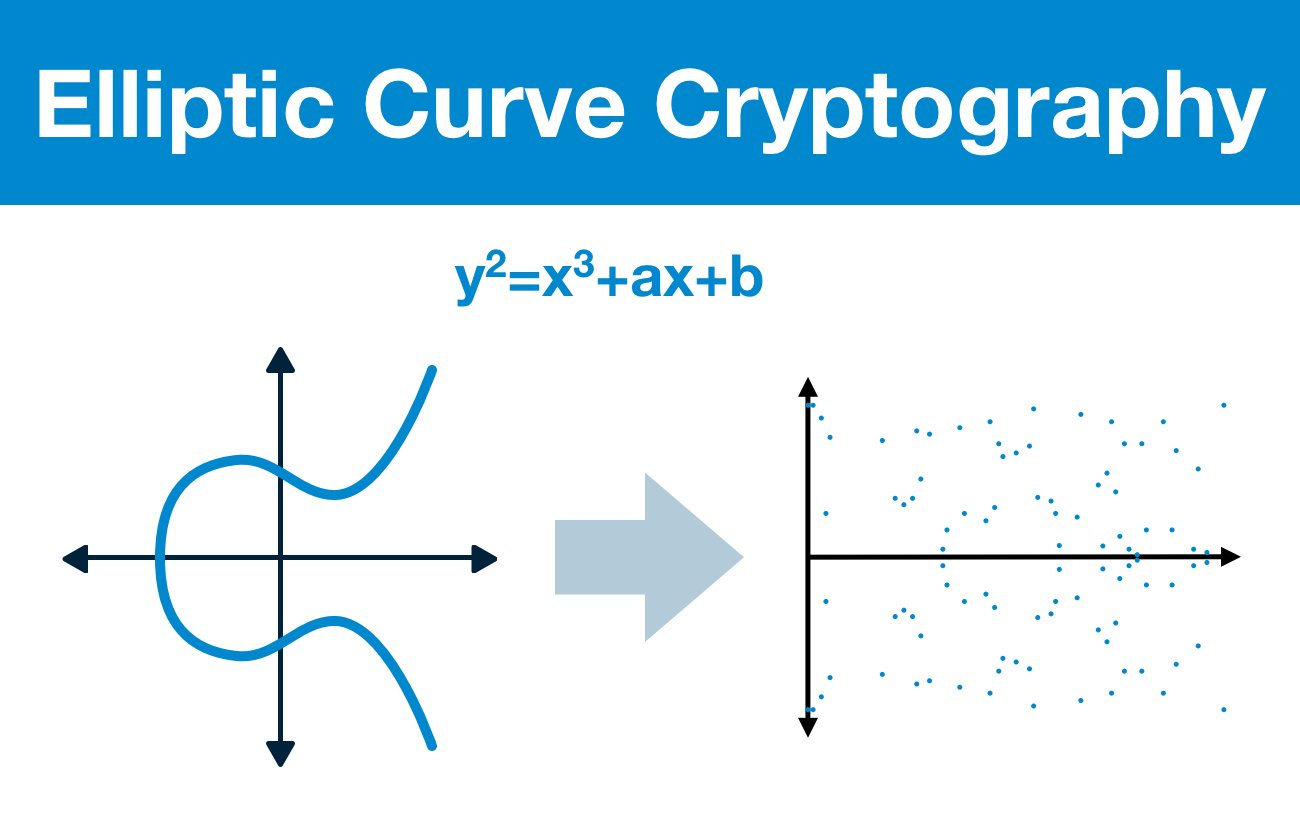
\includegraphics[width=1\textwidth]{\FIGURES/elliptic-curve-cryptography-1.jpeg}
    \caption{Eliptická křivka znázorněna matematickou funkcí. Zdroj: \parencite{eliptic-curve-1}}
    \label{fig:elliptic-curve-cryptography}
  \end{figure}
\newpage
%Hybridní šifry
\section{Hybridní šifry}
\label{sec:hybridni-sifra}

Hybridní šifrovací systémy, jak již vyplývá z jejich názvu, kombinují výhody symetrického a asymetrického šifrování. Tento přístup umožňuje využít silné stránky obou typů šifer, přičemž zajišťuje efektivitu a bezpečnost.
Základní princip hybridních systémů spočívá v tom, že zpráva je šifrována pomocí symetrického šifrovacího algoritmu, který je velmi efektivní při šifrování velkých objemů dat. Symetrický klíč, který byl použit k šifrování zprávy, je následně zašifrován pomocí asymetrického šifrování, a může být bezpečně přenesen mezi odesílatelem a příjemcem. Po obdržení zašifrovaného symetrického klíče ho příjemce dešifruje pomocí svého soukromého klíče a následně použije tento klíč k dešifrování samotné zprávy \parencite{pavlicek2012}.

V praxi se tak s hybridními šifrovacími systémy nejčastěji setkáme pro zabezpečení různých typů komunikace, včetně SSL/TLS~protokolů. Asymetrické metody, které jsou časově náročné slouží k navázání prvního důvěryhodného spojení, zatímco symetrické šifry zajišťují samotné šifrování přenášení velkých bloků dat. Dalším významným využitím je e-mailová bezpečnost, kde technologie jako PGP~a~S/MIME~umožňují šifrování a digitální podepisování zpráv, čímž zaručují, že odesílatel je věrohodný a obsah zprávy nebyl během přenosu změněn \mbox{\parencite{sedlak2021}.}

\subsection{Využití hybridních šifer}

Prvním z příkladů hybridních šifrovacích systémů jsou protokoly SSL~(Secure Sockets Layer) a TLS~(Transport Layer Security). V současnosti se časteji setkáme s protokolem TLS~(verze 1.3) jenž spojuje výhody symetrického a asymetrického šifrování a zajišťuje bezpečnou komunikaci na internetu. Proces navazování bezpečného spojení mezi klientem (např. webovým prohlížečem) a serverem se nazývá \emph{TLS~Handshake}. 

Prvním krokem je, že klient obdrží veřejný klíč serveru, který je obvykle zaslán prostřednictvím digitálního certifikátu podepsaného certifikační autoritou (dále jen CA). Certifikační autorita je důvěryhodná strana, která má pravomoc určit to, že majitel webové stránky je opravdu ten, za kterého se skutečně vydává. Kopii certifikátu si CA~uchovává jen na určitou dobu \parencite{cloudflare2024}. Na vypršení platnosti certifikátu serveru nás nejčastěji upozorní náš webový prohlížeč a zobrazí nám dobře známou hlášku \enquote{Vaše připojení není soukromé}. 
Po dokončení procesu TLS~handshake, používají obě strany stejné \emph{session~keys} (klíče relace) pro šifrování dat. Jakmile jsou klíče relace aktivní, veřejné a soukromé klíče již nejsou dále používány, jelikož~nejsou nutné k ověření autenticity. Klíče relace jsou dočasné klíče, které jsou využívány pouze během jedné relace a po jejím ukončení již nejsou znovu použity. Pro každou novou relaci je vytvořen nový, náhodně generovaný pár klíčů relace.

\begin{figure}[htbp]
    \centering
    
\includegraphics[width=0.8\textwidth]{\FIGURES/symmetric-encryption.jpg}
    \caption{Schéma symetrického šifrování. Zdroj: \parencite{cloudflare2024}}
    \label{fig:symmetric-encryption}
\end{figure}

Existují však i jiné způsoby relace, například v případě takzvaného \emph{session~resumption} (obnovení~relace). Tento mechanismus umožňuje serveru uchovávat šifrovací klíče po určitou dobu, čímž se eliminuje nutnost opětovného provádění celého TLS~handshake při každém novém spojení.

Podle dokumentace GnuTLS \textcite{gnutls2024}, existují dva hlavní způsoby obnovení relace:
\begin {enumerate}
\item \textit{Session~ID} - Server při prvním spojení klientovi přiřadí jedinečný identifikátor relace a dočasně uchová odpovídající šifrovací klíče. Při opětovném připojení klient odešle tento identifikátor a pokud server klíče stále uchovává, může relaci obnovit bez potřeby nového handshake.
\item \textit{Session~Tickets} - Místo aby server uchovával klíče, zašifruje je a pošle klientovi ve formě tzv. session ticketu. Při dalším spojení klient odešle ticket zpět serveru, který jej dešifruje a obnoví relaci. Tento přístup zlepšuje škálovatelnost, protože snižuje zátěž serveru spojenou s ukládáním velkého množství session~keys.
\end {enumerate}

Použití těchto metod nejen zvyšuje výkon a snižuje latenci při opakovaných připojeních, ale také umožňuje efektivnější správu šifrovacích operací, zejména u serverů s vysokým provozem. Nicméně, uchovávání klíčů delší dobu přináší i určitá bezpečnostní rizika - například pokud by došlo k úniku session keys, mohlo by to vést k dešifrování dříve zachycené komunikace (forward~secrecy).
Proto moderní verze TLS~, jako TLS~1.3, preferují ephemeral~key~exchange (pomíjivou výměnu klíčů), kde jsou klíče generovány pro každou relaci zvlášť a historii komunikace již tak nelze zpětně získat \parencite{gnutls2024}. 

Druhým příkladem hybridního šifrovacího systému je technologie~S/MIME, která se využívá pro zabezpečení e-mailové komunikace. Při použití S/MIME odesílatel nejprve digitálně podepíše email svým soukromým klíčem, čímž zajistí, že příjemce může ověřit autenticitu zprávy pomocí veřejného klíče odesílatele. Současně se pro samotné šifrování obsahu zprávy využívá symetrický klíč, který je následně bezpečně předán příjemci za použití asymetrického šifrovacího algoritmu. Tímto způsobem se spojují výhody asymetrické kryptografie a efektivity symetrického šifrování.
Výsledkem je systém, který nejen-že chrání důvěrnost odeslaných zpráv, ale také zaručuje integritu a nepopiratelnost komunikace mezi odesílatelem a příjemcem. Tento přístup se osvědčuje zejména v korporátním prostředí a v aplikacích, kde je klíčová bezpečnost e-mailové komunikace \parencite{cloudflare2024}.

\newpage
%Postkvantová kryptografie
\section{Postkvantová kryptografie}
\label{sec:postkvantova-kryptografie}
V posledních letech rostou obavy, že kvantové počítače, které mají potenciál řešit složité problémy exponenciálně rychleji než klasické počítače, mohou představovat vážnou hrozbu pro současné šifrovací algoritmy. Kvantové počítače využívají jevy, jako je kvantová superpozice a kvantové provázání, což jim umožňuje zpracovávat informace způsobem, který je pro klasické počítače nedosažitelný. Tato schopnost by mohla ohrozit bezpečnost asymetrických šifrovacích algoritmů, jako jsou RSA nebo DSA, které zajišťují bezpečnost většiny online komunikace a které by mohly být kvantovými počítači prolomeny během několika minut\mbox{\parencite{qubits2024}.}

Podle některých odborníků je však tento problém ještě vzdálený 5--15 let, i když se již vyskytují první velké pokroky v této oblasti. Například Google nedávno představil kvantový čip Willow, který je schopen provádět výpočty, jež by pro současné superpočítače byly nedosažitelné. Nicméně tento čip má zatím pouze 105 fyzických qubitů, což je stále daleko od milionů qubitů potřebných k prolomení moderních šifrovacích standardů, jako je RSA. Odhady naznačují, že prolomení RSA šifrování pomocí kvantových počítačů je vzdálené minimálně deset let a vyžadovalo by přibližně 4~miliony fyzických qubitů\parencite{qubits2024}.

V této kapitole budou stručně naznačeny hrozby a výzvy, které kvantové počítače přinášejí pro současnou kryptografii, a budou diskutovány současné snahy o vývoj postkvantových kryptografických algoritmů, které by měly zajistit bezpečnost dat i v oblasti kvantových výpočtů.

\subsection{Shorův algoritmus}
Shorův algoritmus je algoritmus navržený specificky pro kvantové počítače. Algoritmus jenž má za cíl efektivní faktorizaci velkých čísel, vytváří budoucí hrozbu pro bezpečnost šifer, jako je RSA, a tím i šifry, které spoléhají na tento matematický NP-úplný problém.

Nejnovější výzkumy ukazují, že Shorův algoritmus je stále ve fázi experimentálního vývoje. Ačkoliv byl algoritmus navržen pro kvantové počítače s tisíci qubity, první experimenty dosáhli pokroku na menších číselných příkladech. Například studie z roku 2021 popisuje funkční koncept Shorova algoritmu implementovaného na kvantovém počítači s pouhými 7 qubity, kde byl úspěšně proveden rozklad čísla \[N = 21\] na prvočísla. Tento důkaz konceptu ukazuje, že efektivní implementace \mbox{Shorova} algoritmu je prozatím možná jen pro malá čísla \(N\), s malým počtem q-bitů \mbox{\parencite{skosana2021}.}

V současné době je významnou událostí v oblasti postvantové kryptografie, zveřejnění prvních třech standardů (kandidátů) pro postkvantovou kryptografii dle institutu~NIST. Zveřejněné algoritmy by mohly představovat bezpečnou ochranu šifrovaných dat před výpočetní mohutností budoucích kvantových počítačů. Standardy jsou navrženy pro dva klíčové typy aplikací: obecné šifrování pro zabezpečení dat během přenosu a digitální podpisy pro ověřování identity \parencite{nist2024}.

\subsection{Michel Mosca theorem}
Michele Mosca je známý matematik a informatik, který aktuálně působí jako profesor na Univerzitě ve Waterloo (USA) a je spoluzakladatelem fakulty zaměřené na kvantovou výpočetní techniku. Dosud v průběhu své kariéry významně přispěl do výzkumu v této oblasti \parencite{mosca2023}.

Za zmínku stojí právě následující rovnice \textcite{mosca2023}, která upozorňuje na fakt, že bezpečnost současných šifrovacích systémů závisí na překryvu životnosti těchto systémů a nástupu kvantových počítačů:
\begin{equation}
X + Y > Z
\end{equation}
kde:
\begin {description}
\item[$Z$] - Doba, za kterou bude k dispozici efektivní kvantový počítač.
\item[$Y$] - Doba potřebná k implementaci kvantově odolné šifry pro stávajicí systém.
\item[$X$] - Doba, po kterou chceme tajnou informaci uchovat v utajení.
\end {description}
\newpage

%Seznam literatury
\newpage
\section*{Seznam literatury}
\addcontentsline{toc}{section}{Seznam literatury}
\printbibliography[heading=none]

%Seznam obrázků
\newpage
\listoffigures  

\end{document}
